\chapter{Optical Lattice Potentials}
Cold atoms can be trapped in potentials generated through their own dipole interaction with light. Thus, superimposing laser beams allows one to create optical lattices in various shapes and forms. The lattice does not only trap the atoms, its properties and periodic nature is also reflected its corresponding states. Creating such a lattice and loading the cold atoms into it is one of the initial step of many experiments. 

\section{Trapping of Neutral Atoms}
Neutral atoms can be trapped through the dipole potential induced by atom-light interaction. Consider a two level atom in the presence of a time-varying electric field $\boldsymbol{E} = \boldsymbol{\varepsilon} E_0 \exp{ \left( i(\boldsymbol{k} \boldsymbol{r} - \omega_L t) \right)}$, where $E_0$ is its amplitude, $\boldsymbol{\varepsilon}$ is its polarization vector, $\boldsymbol{k}$ is its wave vector and $\omega_L$ is its frequency. The interaction between the atom and the E-field will lead to a perturbation of the energy levels, otherwise known as the AC Stark-shift. The Hamiltonian describing this interaction is
\begin{equation}
	\hat{H}_{int} = \hat{d} \boldsymbol{E} \; ,
\end{equation}
where $\hat{d} = -e \hat{r}$ is the electric dipole operator.\\
This interaction can be seen as a perturbation to the atoms Hamiltonian. To first order the non-degenerate, time-independent perturbation of the energy of state $i$ reads $E_{i}^{(i)} = \bra{i} \hat{H}_{int} \ket{i}$. However, only states of opposite parity will contribute to the matrix elements of $\braket{\hat{H}_{int}}$, thus leaving the first-order perturbation terms zero.\\
To second order the perturbation of state $i$ is given by
\begin{equation}
	E_i^{(2)} = \sum_{j \neq i} \frac{ |\bra{j} \hat{H}_{int}\ket{i}|^2}{\varepsilon_i - \varepsilon_j} \; .
\end{equation}
Here, $\ket{i}$ and $\ket{j}$ are states of the combined system of the two-level atom and the light field. The state $\ket{i}$ represents the atom being in its ground state, while the light field contains $n$ photons. Thus, the energy of the combined state is $\varepsilon_i = n \hbar \omega_L$, when setting the energy of the atomic ground state to zero. Meanwhile, state $\ket{j}$ is when the atom has been excited by absorbing one of the photons of the field. Hence, the energy of this state is $\varepsilon_j = \hbar \omega_0 + (n-1) \hbar \omega_L$. Defining the detuning $\Delta = \omega_L - \omega_0$ allows writing the perturbation in the form
\begin{equation}
	E_{g/e}^{(2)}=\pm  \frac{ |\bra{e}\hat{d}\ket{g}|^2}{\Delta} |E_0|^2,
	\label{2ndpert}
\end{equation}
where the upper sign is assigned to the atomic ground state $\ket{g}$. This can be rewritten in order to reflect properties of the atom and the field, by writing it using the intensity of the light, $I = \frac{1}{2} \epsilon_0 c |\boldsymbol{E}|^2 $, and the decay rate of the atom, $\Gamma$. Thus, equation \ref{2ndpert} can be written as \cite{grimm} 
\begin{equation}
	E_{e/g}^{(2)}=\pm \frac{3 \pi c^2}{2 \omega_0} \frac{\Gamma}{\Delta}I
	\label{eq:dipolepot}
\end{equation}
This is the AC-Stark shift, which constitutes the dipole potential. For red detuning ($\Delta < 0$) the ground state will experience a negative shift leading to an attractive potential with depth depending on the intensity of the laser. Similarly, a blue-detuned laser will repel the atom. An illustration of this can be seen in figure \ref{fig:ac_stark}.
\begin{figure}[!h]
	\centering
	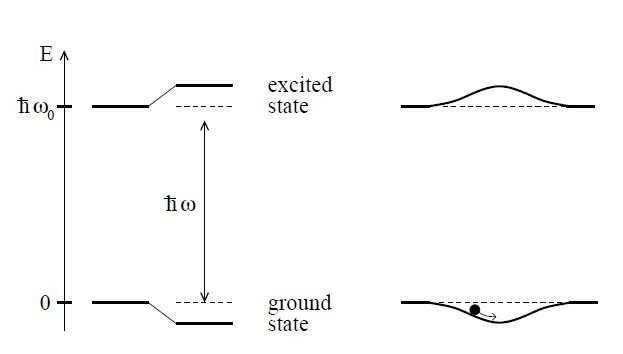
\includegraphics[width=0.5\columnwidth]{Figures/acstark.JPG} 
	\caption{\textit{Light shifts of a two-level atom. Left-hand side,
		red-detuned light ($\Delta < 0$) shifts the ground state down and the
		excited state up by same amounts. Right-hand side, a spatially
		inhomogeneous field like a Gaussian laser beam produces a
		ground-state potential well, in which an atom can be trapped. The figure and 		caption are adopted from \cite{grimm}.}}
	\label{fig:ac_stark} 
\end{figure}
Since the sign is reversed for the excited state, it is important that the atom remains in the ground state. Thus, one has to minimize the scattering with the optical potential. The scattering rate is given as \cite{grimm}
\begin{equation}
	\Gamma_{sc} = \frac{3 \pi c^2}{2 \hbar \omega_{0}^3} \left( \frac{\gamma}{\Delta} \right) I \; .
\end{equation}
Therefore, one has to choose a large detuning in order to reduce the scattering rate. However, this comes at the cost of a weaker potential. Hence, a large intensity must be used to compensate the detuning, such the potential can achieve sufficient depth.


\section{Optical Lattices}

The dipole potential in equation \ref{eq:dipolepot} scales with the intensity of the laser. Thus, superimposing laser beams allows for creating a multitude of different potentials. A simple standing wave will lead to an array of potential wells
\begin{equation}
	V(z) = - V_0 \cos^2{k z } \; ,
	\label{eq:standwave}
\end{equation}
 where $V_0 = | \frac{3 \pi c^2}{2 \omega_{0}^3} \frac{\Gamma}{\Delta} 4 I_0 |$. In practise, a one dimensional lattice like that of equation \ref{eq:standwave} is created by shining a single laser beam at a mirror, thus interfering with itself creating a standing wave.
\begin{figure}[!h]
	\centering
	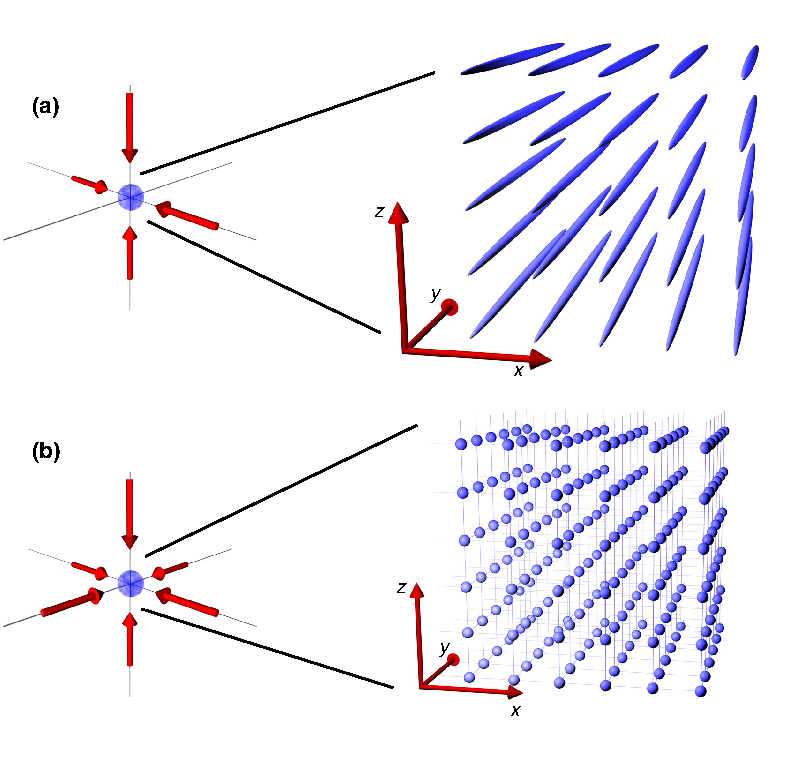
\includegraphics[width=0.8\columnwidth]{Figures/OpticalLattice.pdf} 
	\caption{\textit{\textbf{(a)} Two dimensional optical lattice formed by two mutually orthogonal laser beams. These tubes have a characteristic cigar shape, due to the Gaussian profile of the lasers. \textbf{(b)} Upon using three orthogonal laser beams, the result is a three dimensional lattice reminiscent of a cubic crystal. Figure is adopted from \cite{WideraThesis}.}}
	\label{fig:OpticalLattice} 
\end{figure}
Adding another laser beam in a different direction creates a periodic two dimensional potential. For orthogonal polarization of the two lasers, the resulting potential is purely the sum of the sinusoidal standing wave potential, as no interference term is present \cite{lewenstein}. Note, that the lattice is only well defined for distances much smaller than the waist of the laser beams, as the lattice is only present within the overlap of the two beams. Various shapes of the lattice can be achieved by adjusting the angle between the beams, however, the most common setup is using two orthogonal beam creating a square lattice of one dimensional tubes, as seen in figure \ref{fig:OpticalLattice}.
In order to create a three dimensional lattice as seen in figure \ref{fig:OpticalLattice}, an additional third perpendicular laser beam is needed. In center of the trap, the lattice potential is then given by
\begin{equation}
	V(x,y,z) = - V_0 \left( \cos^2{k x } + \cos^2{k y } + \cos^2{k z } \right) \; ,
\end{equation}
for distances much smaller than the beam waist. In addition to the lattice an external harmonic confinement will be present due to Gaussian profile of the laser beams \cite{manybodyBloch}.

\section{Band Structure}
Consider a periodic potential as described by equation \ref{eq:standwave}. \textit{Bloch's Theorem} states that energy eigenstates of a periodic potential with lattice vector $\boldsymbol{R}$ and quasi-momentum $q$ can be written as Bloch waves, which takes the form
\begin{equation}
	\phi_{\boldsymbol{q}}^{(n)}(\boldsymbol{r}) = e^{i \boldsymbol{q} \boldsymbol{r}} u^{(n)}(\boldsymbol{r}) \; ,
\end{equation}
which is a plane wave modulated by a function with the same periodicity as the potential $u^{(n)}(\boldsymbol{r}) = u^{(n)}(\boldsymbol{r} + \boldsymbol{R})$. Furthermore, the Bloch waves are periodic in reciprocal space, such that $\psi_{\boldsymbol{q}}^{(n)}(\boldsymbol{r}) = \phi_{\boldsymbol{q} + \boldsymbol{G}}^{(n)}(\boldsymbol{r})$, where $\boldsymbol{G}$ is a reciprocal lattice vector. \cite{kittel} \\
This leads to an energy spectrum in the shape of bands with the periodicity of the first \textit{Brillouin Zone}. Bands are denoted by the band index $n$, and their shape is determined by both the shape and the depth of the potential.\\
The potential depth is often denoted in units of the recoil energy $E_r = \frac{\hbar ^2 k^2}{2 m}$, where $m$ is the mass of the atom, and $k$ is the photon wave number of the light forming the optical lattice. For $V_0 = 0$ the particles are free, hence the bands will be parabolic. Meanwhile, for $V_0 \rightarrow \infty$ no interactions between different wells of the lattice can take place, as the wavefunctions of the trapped atoms will be confined to their respective well. Thus, the lattice is reduced to an array of independent harmonic oscillators, whereby the bands will appear flat with equal spacing \cite{greiner}. 

\section{Localized States}
For lattice potential depths within $5 E_r \leq V_0 \leq 8 E_r$, the lattice is in the \textit{tight binding limit}. Within this range, the wavefunctions of the trapped atoms will only overlap with other wells in their closest proximity. Thus, interactions between wells are almost purely of nearest neighbour nature. Due to how well localized the wavefunctions are, a basis of Wannier functions is ideal for describing the system. Wannier functions are related to Bloch functions through the Fourier transform
\begin{equation}
	w^{(n)}(\boldsymbol{r}) = \frac{1}{\sqrt{N_L}} \sum_{q} e^{ -i \boldsymbol{q} \boldsymbol{R} } \phi_{\boldsymbol{q}}^{(n)}(\boldsymbol{r}) \; ,
\end{equation} 
where $N_L$ is the number of primitive cells of the lattice, and $\boldsymbol{R}$ is is a Bravais lattice vector. The Wannier functions are well localized and centered around the lattice at site $\boldsymbol{R}$. Furthermore, they obey the orthonormality relation
\begin{equation}
	\int \mathrm{d^3}r \; \; w^{(n) *}(\boldsymbol{r} - \boldsymbol{R}) w^{(n')}(\boldsymbol{r} - \boldsymbol{R'}) = \delta_{n,n'} \delta_{\boldsymbol{R},\boldsymbol{R}'} \; ,
\end{equation}
thus forming a complete basis \cite{manybodyBloch}.
\begin{figure}[!h]
	\centering
	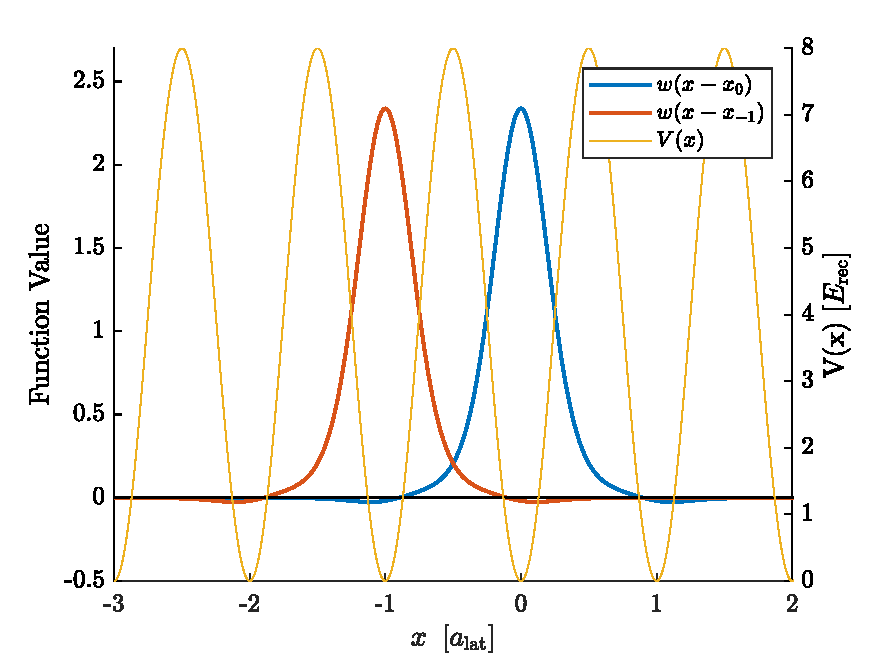
\includegraphics[width=0.8\columnwidth]{Figures/WannierPlot3.pdf} 
	\caption{\textit{Two one-dimensional Wannier functions plotted for a lattice potential depth of $V_0 = 8 E_r$.}}
	\label{fig:WannierPlot} 
\end{figure}
Figure \ref{fig:WannierPlot} shows Wannier functions plotted for lattice potential depths within the tight binding limit. As evident from the plot, the functions overlap with only their nearest neighbours. In the case of a more shallow lattice, the functions would extends to further wells, while they will tend towards a Gaussian shape as the lattice depth increases.